\documentclass[10pt, conference, letterpaper]{IEEEtran}
\usepackage{amsmath}
\usepackage{graphicx}
\usepackage{cite}
\usepackage{booktabs}
\usepackage{url}

\begin{document}
\title{Advanced Topologies of Drivers for Piezoelectric Actuators: Comparative Analysis of Linear and GaN Switched Amplifiers}

\author{
\IEEEauthorblockN{Marek Karlicek}
\IEEEauthorblockA{Faculty of Electrical Engineering and Communication, Department of Physics\\
Brno University of Technology\\
Brno, Czechia\\
marekkarlicek@gmail.com}
}

\maketitle

\begin{abstract}
The development of modern mechatronics, precise positioning, and ultrasonic technologies is inherently linked to the use of piezoelectric actuators. While these elements offer excellent mechanical parameters, the design of their control electronics represents one of the most complex challenges in power electronics. This paper presents a detailed comparative analysis between conventional analog linear Class~AB amplifiers and modern switched Class~D topologies utilizing Gallium Nitride (GaN) wide-bandgap semiconductors. The physical model of the piezoelectric load is discussed based on real impedance measurements, revealing its frequency-dependent capacitive and resonant nature. Furthermore, the paper details the digital control infrastructure utilizing an STM32 microcontroller and high-resolution timer (HRTIM) to synthesize precise voltage waveforms. The transition to GaN-based full-bridge topology enables energy recuperation, significantly increasing system efficiency to over 90\% and minimizing thermal dissipation typical for linear operating regions.
\end{abstract}

\begin{IEEEkeywords}
Piezoelectric Actuators, Gallium Nitride (GaN), Class~D Amplifier, Linear Amplifier, Power Electronics, vibration analysis, STM32, HRTIM
\end{IEEEkeywords}

\section{Introduction to Piezoelectric Actuator Driving and Research Context}
Piezoelectric materials offer excellent mechanical properties—sub-nanometer resolution, extreme dynamic response, and significant force generation. In this work, the principal motivation is the excitation of controlled vibrations in metallic structures to study acoustic wave propagation. This demands precise voltage waveforms, high timing control (nanosecond-scale), and excellent repeatability.

Although the piezoelectric actuators themselves offer excellent mechanical parameters \cite{ieee_std_piezo}, the design of their control electronics represents one of the most complex problems in the field of power electronics. From an electrical circuit perspective, a piezoelectric actuator appears predominantly as a highly capacitive load. This capacitance can range from hundreds of picofarads in tiny positioning crystals to tens of microfarads in large multilayer piezoelectric stacks. Moreover, achieving full mechanical displacement requires very high driving voltages, typically ranging from tens to hundreds of volts (e.g., $\pm 150$\,V to $400$\,V).

For low-power applications, such as tactile feedback and haptics in mobile consumer electronics, semiconductor manufacturers have introduced dedicated monolithic piezoelectric drivers (e.g., Texas Instruments DRV2667 \cite{ti_drv2667} or specialized energy-recovery ICs from Bor\'{e}as Technologies \cite{boreas_bos1901}). These highly integrated chips typically employ a built-in boost converter followed by a low-voltage Class AB or rudimentary Class D amplifying stage. However, while exceptionally compact and suited for short transient pulses, they are fundamentally limited in continuous output power and voltage swing. Thus, they are insufficient for heavy-duty industrial or high-end mechatronic applications.

With modern wide-bandgap (WBG) semiconductors—particularly Gallium Nitride (GaN)—switched Class~D topologies offer an alternative. By enabling energy recuperation from the capacitive load back to the supply, Class~D amplifiers can achieve system efficiencies exceeding 90\%, compared to below 30\% for linear designs. Furthermore, GaN switching speeds permit megahertz modulation frequencies \cite{HfGan_power_integration}, allowing switched amplifiers to approach the signal fidelity of linear circuits while recovering reactive power.

\section{Physical Nature and Electro-Mechanical Modeling of Piezoelectric Elements}
To make a well-founded comparison of different amplifier topologies, it is first necessary to perfectly understand the load these amplifiers drive. The standard approach for engineering design of electronic circuits is the use of the Butterworth-Van Dyke (BVD) equivalent circuit.

\subsection{Butterworth-Van Dyke (BVD) Equivalent Model}
The BVD model divides the actuator into two parallel branches:
\begin{itemize}
    \item \textbf{Static (Electrical) Branch:} Contains a capacitor $C_0$, referred to as clamped capacitance. It represents the purely geometric capacitance of the dielectric material.
    \item \textbf{Motional (Mechanical) Branch:} Formed by a series connection of inductance $L_1$, capacitance $C_1$, and resistor $R_1$. These represent effective inertial mass, mechanical compliance, and internal mechanical losses respectively.
\end{itemize}

The impedance of the entire BVD circuit $Z(\omega)$ as a function of angular frequency $\omega = 2\pi f$ is given in \cite{bvd_model_analysis} as:
\begin{equation}
Z(\omega) = \frac{1}{j\omega C_0 + \frac{1}{R_1 + j\omega L_1 + \frac{1}{j\omega C_1}}}
\label{eq:bvd_impedance}
\end{equation}

\subsection{Analysis of Real Impedance Characteristics}
Real impedance characteristics were measured using a Keysight E4990A precision impedance analyzer \cite{keysight_e4990a}.

% Placeholder pro vlozeny graf z Pythonu (Trace02.csv)
\begin{figure}[htbp]
\centerline{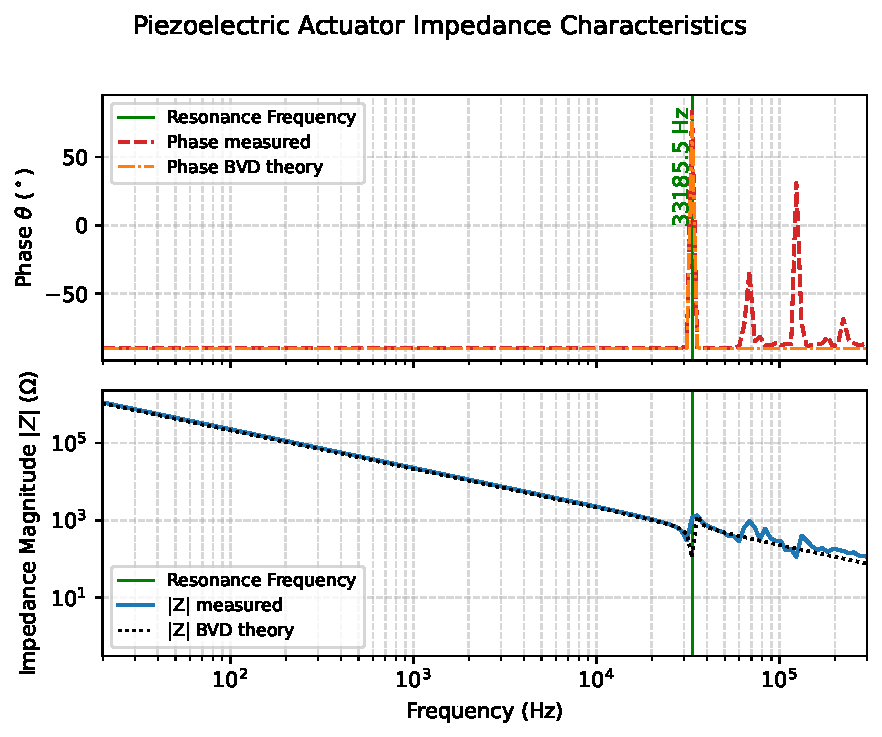
\includegraphics[width=1\columnwidth]{src/impedance_graph.pdf}}
\caption{Measured impedance magnitude and phase of the piezoelectric actuator; the series-resonant frequency is marked (Keysight E4990A data).}
\label{fig_impedance}
\end{figure}

In the low-frequency region below resonance, the impedance magnitude drops logarithmically with increasing frequency, and the phase holds strictly around -90$^{\circ}$. The load capacitance remains constant at an average value of approximately 7.05\,nF. This proves that below resonance, the motional branch of the BVD model exhibits no activity, and the entire actuator behaves as an ideal capacitor.

Around the series-resonant region, the impedance reaches a local minimum and the phase transitions rapidly, indicating a shift from predominantly capacitive behavior toward a more resistive/inductive response. Near anti-resonance, the impedance increases toward a local maximum. Even without full-curve overlay in Fig. \ref{fig_impedance}, the measured resonance behavior has direct implications for amplifier design: off-resonance driving is predominantly reactive, operation near resonance approaches a higher resistive contribution ($R_1$).

The calculated equivalent-circuit values for the measured actuator are summarized in Table \ref{tab:bvd_params}.

\begin{table}[htbp]
\centering
\caption{Calculated BVD model parameters}
\label{tab:bvd_params}
\begin{tabular}{@{}llrl@{}}
\toprule
\textbf{Parameter} & \textbf{Symbol} & \textbf{Value} & \textbf{Unit} \\
\midrule
Static capacitance & $C_0$ & 7.03 & nF \\
Motional capacitance & $C_1$ & 0.53 & nF \\
Motional inductance & $L_1$ & 43.85 & mH \\
Motional resistance & $R_1$ & 15.20 & $\Omega$ \\
\midrule
Effective coupling factor & $k_{eff}$ & 0.26 & - \\
\bottomrule
\end{tabular}
\end{table}

\section{Linear Amplification Concept: Class AB Topologies and Apex Circuits}
The first of the two realized amplifiers utilizes a classical linear topology, based on high-voltage power operational amplifiers (e.g., Apex Microtechnology models like PA92 or PA107) \cite{apex_pa92,apex_pa107}.

\subsection{Stability Issues with Capacitive Loads}
Voltage amplifiers with negative feedback are inherently prone to instability when driving large capacitive loads. The load capacitance forms an RC low-pass filter with the op-amp's output impedance, introducing an additional pole into the open-loop transfer function. Compensation networks e.g., a series isolation resistor ($R_{ISO}$) or more sophisticated Dual-Feedback loops, must be deployed to ensure high-frequency stability without compromising DC static accuracy. Because the feedback loop forces the output voltage to track the input reference exactly, it inherently provides excellent Power Supply Rejection Ratio (PSRR).

\subsection{Power Losses and Thermal Analysis}
A fundamental drawback of linear driving is the immense energy inefficiency. For sinusoidal driving into a purely capacitive load, the average power dissipated on the amplifier transistors is given by:
\begin{equation}
P_{diss} = \frac{4 \cdot V_{supply} \cdot V_{p} \cdot \omega \cdot C_{load}}{\pi}
\label{eq:power_dissipation}
\end{equation}
This massive thermal dissipation  \eqref{eq:power_dissipation} from strictly necessitates the use of large aluminum heatsinks, limiting the potential for miniaturization and mobile system deployment \cite{apex_linear}.

\section{Switched Drivers based on GaN Half-Bridges (Class D)}
Due to the thermal constraints of linear systems, wide-bandgap (WBG) materials, primarily Gallium Nitride (GaN), have come to the forefront of switched topology implementations.

\subsection{Full-Bridge (BTL) Topology and Recuperation}
The switched amplifier connects two integrated GaN half-bridges (forming a Full-Bridge or Bridge-Tied Load structure). The load is connected differentially between the outputs, doubling the effective voltage swing.
In the presented switching arrangement, the upper transistor of one half-bridge is driven together with the lower transistor of the opposite half-bridge (diagonal pairing), while the complementary diagonal pair is switched in the opposite state. This corresponds to bipolar full-bridge switching as depicted in Fig. \ref{fig_gan_sch}.

In practical hardware, this concept can be implemented using compact integrated GaN power stages, for example devices from the Navitas GaNFast family. A representative example is the NV6247C \cite{navitas_nv6247c}, which is intended for high-frequency half-bridge operation and integrates the fast GaN switching devices together with the associated gate-drive and protection infrastructure into a single compact power IC. Using two such half-bridge modules simplifies the realization of a full-bridge piezo driver, reduces parasitic loop inductance compared with a discrete implementation, and helps preserve the fast switching edges required for efficient operation.

The key component is the output LC low-pass filter. When the capacitive piezoelectric load discharges, the LC filter and the switched-on transistors create a recuperation path, directing the current back into the primary bulk capacitors on the supply rail. Reactive energy loss is minimized, elevating system efficiency to 90--95\%.

% Placeholder pro schema spinaneho GaN zapojeni
\begin{figure}[htbp]
\centerline{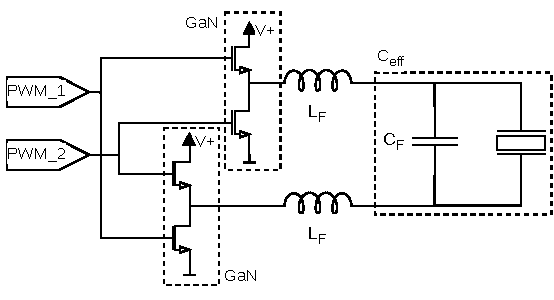
\includegraphics[width=0.85\columnwidth]{src/GAN_block.pdf}}
\caption{Circuit architecture of the Gallium Nitride (GaN) based full-bridge switched Class D amplifier.}
\label{fig_gan_sch}
\end{figure}

\subsection{EMI and Dead-Time Considerations}
High $dv/dt$ transients (for tested GaN NV6247C  up to 100\,V/ns) induce significant electromagnetic interference (EMI). Moreover, a perfectly calibrated dead-time (the nanosecond-scale delay preventing shoot-through) is necessary. GaN technology enables dead-time reduction to under 5\,ns, thus approximating the purity of analog reproduction without losing phenomenal energy efficiency.
\subsection{Linearity and the (Non)Necessity of Feedback}
A critical parameter in power amplifiers is linearity. Unlike Class~AB amplifiers, where feedback is mandatory to suppress crossover distortion and stabilize gain, Class~D topologies suffer from non-linearities primarily dictated by dead-time duration, switching delays, and finite device on-resistance. In traditional audio Class~D applications, complex analog feedback loops---taken either before or after the LC filter---are implemented to correct these distortions and improve the Power Supply Rejection Ratio (PSRR).

However, in the context of driving highly reactive and resonant piezoelectric actuators, implementing a real-time analog feedback loop across an LC filter poses severe stability risks and degrades the inherent efficiency of the Class~D driver. The combination of the multi-order LC network and the highly frequency-dependent impedance of the piezo element (per the BVD model) creates complex pole-zero structures leading to immense phase shifts. Operating purely in open-loop sacrifices PSRR, meaning the output stage becomes directly dependent on the supply rail stability. However, due to the nearly ideal switching characteristics of GaN devices (nanosecond-scale dead-time, very low $R_{DS(on)}$, and zero reverse recovery charge $Q_{rr}$), the open-loop linearity of the power stage is natively exceptionally high. Therefore, closed-loop analog feedback becomes largely redundant and often counterproductive. Any residual structural non-linearities of the piezoelectric displacement are more efficiently compensated in the digital domain through mathematical pre-distortion of the modulation signal (feed-forward control) rather than risking hard-to-tame oscillations with an analog feedback loop. Consequently, the GaN driver operates reliably in an open-loop configuration.

\subsection{LC Output Filter Design and Voltage Ripple}
The output LC low-pass filter ($L_f$, $C_f$) is unequivocally the most critical passive subsystem of the Class~D topology. Its primary function is to demodulate the high-frequency PWM switching signal back into the desired analog baseband waveform while attenuating the switching frequency carrier ($f_{sw}$) to bound the output voltage ripple ($\Delta V_{out}$).

The theoretical cutoff frequency $f_c$ of the second-order LC filter is defined in \cite{LC_filter_design} as:
\begin{equation}
f_c = \frac{1}{2\pi\sqrt{L_f C_f}}
\label{eq:lc_cutoff}
\end{equation}
However, when driving piezoelectric actuators, the clamped capacitance of the actuator ($C_0$), running in parallel with the filter's physical capacitor, must be strictly accounted for. The effective cutoff frequency thus shifts lower to $f_{c,eff} = [2\pi\sqrt{L_f (C_f + C_0)}]^{-1}$.

The selection of $L_f$ and $C_f$ represents a fundamental trade-off between the amplifier's control bandwidth and the residual high-frequency voltage ripple. Assuming a full-bridge (BTL) topology with bipolar PWM switching, the maximum peak-to-peak voltage ripple (occurring at a 50\% duty cycle) can be approximated as in \cite{LC_filter_design}:
\begin{equation}
\Delta V_{out} \approx \frac{V_{supply}}{16 L_f (C_f + C_0) f_{sw}^2}
\label{eq:ripple_estimate}
\end{equation}
Driving the GaN device at elevated switching frequencies ($f_{sw}$ in the MHz range) allows for a drastic reduction in $L_f$ and $C_f$ values \cite{LC_filter_design}. This not only minimizes the physical footprint and equivalent series resistance (ESR) losses of the inductors but also pushes the LC pole far beyond the mechanical resonance frequencies of the piezoelectric element. Consequently, this prevents unpredicted structural excitation and destructive delamination of the piezoceramic stack caused by switching harmonics.

\section{Firmware Infrastructure and Signal Generation (STM32 HRTIM)}
Precise positioning demands an ultra-fast digital control system capable of synthesizing PWM signals in the megahertz range with nanosecond resolution. The STM32H7 microcontroller utilizing the HRTIM (High-Resolution Timer) peripheral \cite{stm32_hrtim}, DMA, and LwIP networking stack performs this task effectively. The HRTIM directly fetches up to 16-bit payload values via DMA to dynamically manipulate the timer compare register values (CMP) cycle by cycle; the corresponding normalized duty cycle is given by $d = CMP/PER$. In this sense, the modulator effectively operates as a high-frequency Power-DAC without burdening the primary CPU core.

\section{Waveform Validation and Iterative Tuning}
For the studied application, the practical objective is not generic real-time signal synthesis, but repeated reproduction of a prescribed excitation waveform. In such a scenario, a measurement-driven workflow is more appropriate than assuming a purely predictive software-side correction model. The generated drive signal can be measured directly using an oscilloscope or another sufficiently fast sampling instrument, compared with the desired target waveform, and iteratively refined until the observed output matches the requirement.

This approach is particularly effective when the system repeatedly amplifies a single fixed burst or pulse sequence. Once the response of the complete chain consisting of the PWM modulator, GaN power stage, output filter, interconnect, and piezoelectric load has been measured, the stored excitation vector can be adjusted offline and replayed identically in subsequent experiments. The method therefore shifts the optimization problem from real-time adaptive filtering to offline identification and refinement of a deterministic waveform, which is fully adequate for laboratory excitation of acoustic waves in solid metallic specimens.

The measured transfer behavior between programmed timer compare register values (CMP) and resulting output voltage is shown in Fig. \ref{fig_linearity}; duty cycle can be obtained as $d = CMP/PER$.

\begin{figure}[htbp]
\centerline{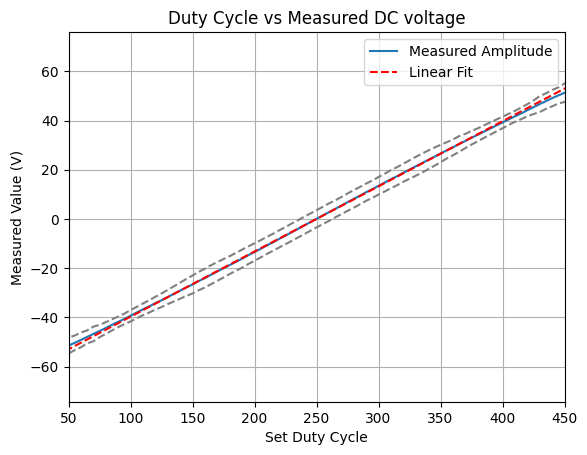
\includegraphics[width=1\columnwidth]{lintest.png}}
\caption{Measured linearity of the output voltage relative to the programmed timer compare register value (CMP) in an open-loop configuration. The dashed curve denotes measured peak-to-peak amplitudes ($V_{pp}$).}
\label{fig_linearity}
\end{figure}
\section{Conclusion}
The design of power electronics for piezoelectric systems is an inherent compromise between signal reconstruction purity and thermodynamic efficiency limits. While analog linear Class~AB amplifiers offer peak linearity, their destructive thermal profile prevents scaling in mobile devices. The GaN-based Class~D full-bridge switches bring a paradigm shift, resolving reactive energy dissipation through active recuperation and negligible switching losses. Precise modulation control via high-resolution timers on modern microcontrollers bridges the gap between digital processing precision and immense power delivery demands. In the demonstrated use case, this architecture provides a practical platform for injecting repeatable mechanical excitation into a metallic structure and studying the propagation of the resulting acoustic wave under controlled electrical drive conditions.

\bibliographystyle{IEEEtran}
\bibliography{references}

\end{document}
